\documentclass[11pt]{article}

\usepackage[english]{babel}
\usepackage[T1]{fontenc}
\usepackage[utf8]{inputenc}
\usepackage{mathtools}                       % matma
\usepackage{amsfonts,amsmath,amssymb,amsthm} % matma
\usepackage{braket}
\usepackage{tikz}

\title{Computational Complexity, homework problem 2, Fall 2024}
\author{Stanisław Bitner}
\date{\today}

\begin{document}
\maketitle

\section{Problem 2.1}

\subsection{Checking if $T_1$ and $T_2$ are trees}
One of the definitions of tree $T = (V,E)$ is that $T$ must be connected and
$|V| = |E| + 1$. It has been said during the lecture that checking connectivity
of a graph can be done in $L$. Checking if $|V|=|E|+1$ is trivial to do by
counting separators between vertices on one counter and separators between edges
on another counter. Afterwards it is enough to ensure that counter$_1$
- counter$_2$ = $1$. We check this for both $T_1$ and $T_2$. Unless both of them
satisfy the conditions, we reject.

\subsection{Denoting vertices}
As it is impossible to hold vertices on a tape in $L$, we will be storing their
indices on the input tape. To compare 2 vertices $v, u$ and know whether they
are equal or not we compare their indices. To find index $i$ of vertex $v$ is
trivial and can be done using 3 counters: one at start of the tape, one for
index starting with 0, one pointing at current vertex. We increment 1st counter
by 1 until it is equal to 3rd counter. We increment 2nd counter each time we
encounter a vertex separator with the 1st counter. Afterwards we move 1st
counter to the start of the tape and copy 2nd counter to the counter that we
want to store the index of vertex $v$.\\
Another problem would be comparing vertices that are in edges of the graph. We
combat this by once again using a few counters: one counter at the start of the
tape, one for index starting with 0, one pointing to the beginning of the vertex
in the input tape. We compare vertices pointed by the 1st and 3rd counters
character by character. If they are equal then we have the index in 2nd
counter. Otherwise, we move 1st counter to the beginning of next vertex and
increment 2nd counter by 1. Then we repeat -- as the input is a correct graph
representation, such algorithm shall terminate.

\subsection{Stack}
First let's define some stack operations.\\ By stack, I mean an array of some
fixed length (let's say $100$) of pairs of counters. First element of each pair
is the index of vertex $v$ from the input tape, the second element is the index
of a set $\{v, u\}$ denoting an edge connecting vertices $v$ and
$u$. Additionally, in state we keep stack's size (it is a constant).\\
Furthermore, let's define some stack operations:
\begin{itemize}
    \item stack.push(v,i) -- increment stack size $s$ by 1. Then put into $s$-th pair
        2 counters: index of vertex $x$ and $i$;
    \item stack.pop(v, i) -- decrement stack size by 1;
    \item stack.size() -- is just a way to denote stack size held in the state;
    \item stack.top() -- this refers to the $s$-th pair of counters held on the stack, $s$ being the stack's size;
    \item stack.empty() -- this is a boolean function true if stack.size() = $0$.
\end{itemize}

\subsection{Finding degree of vertex}
Let deg($v$) be the degree of vertex $v$. We can calculate it in $L$ by using
counters: one pointing at the beginning of $v$ in the input tape, another one
starting at the beginning of the set of edges of the graph, third one for
counting the degree. Then we count number of vertices in the set of edges that
are the same as the vertex pointed by the first counter. We can compare the
vertices as string, character by character.

\subsection{Iterating over neighbours}
To iterate over neighbours of $v$ in $L$ we may hold a counter $l$ being the
index of the last neighbour. We start with $l = 0$. Then we increase the counter
and if we encounter a pair $(v,u)$, $u$ is the neighbour, then we can perform
some operations for $u$ and carry on.

\subsection{Finding T1's diameter}
It is trivial that a tree with radius not greater than $2$ has a diameter of at
most 4, where diameter is the longest path in the tree. Here we want to find the
diameter of $T_1$ whilst also checking if it is not too big. Furthermore, we
observe that the \emph{special} vertex of tree $T_1$ would be the center of the
diameter, because if the diameter does not exceed 5 (counting vertices, not
edges), then the shortest path to each other vertex in $T_1$ would be at most
$2$. It is a well known fact that one way to find a diameter of tree is to
choose an arbitrary vertex as the start. Then find a vertex $s$ furthest to
it. Then we find a vertex $t$ furthest from $v$. The tree diameter is thence
path $v \rightsquigarrow u$.\\
We could describe an algorithm for that as follows:
\begin{enumerate}
    \item Let $s,t,v,u,i$ be counters
    \item s shall represent the $0$-th vertex of $T_1$ (it's the index)
    \item stack.push(s, 0) -- DFS
    \item d := 0 -- longest path; we store it in state as it can only be finite
    \item while not stack.empty():
        \begin{itemize}
            \item $(v,i)$ := stack.top(), stack.pop()
            \item $u$ := $i$-th neighbour of $v$
            \item if $u$ doesn't exist, continue
            \item $p$ := stack.top().first if not stack.empty()
            \item stack.push($v$, $i+1$)
            \item if $p \neq u$, stack.push($u$, $0$)
            \item if stack.size() > $5$, reject as $T_1$ has too large radius
            \item if stack.size() > $d$, $t = u$, $d$ = stack.size()
        \end{itemize}
    \item s := t
    \item repeat DFS with new s, 
    \item diameter of $T_1$ is now $s \rightsquigarrow t$
\end{enumerate}

\subsection{Finding the center}
\begin{enumerate}
    \item Let $c$ be a counter
    \item perform DFS again from $s$, but break after pushing $t$ to the stack
    \item do stack.pop() $\lfloor \frac{d}{2} \rfloor$ times
    \item $c$ = stack.top().first
\end{enumerate}

Now vertex $c$ is the \emph{special} vertex described in the problem statement.

\subsection{Checking isomorphism}
The approach we will take is very simple, as the structure of $T_1$ must be
simple. There must exist $c' \in V(T_2)$, such that the following conditions
must be satisfied to accept:
\begin{itemize}
    \item $deg(c) \le deg(c')$;
    \item $\forall_{i \in 1..deg(c)} s_c(i) <= s_{c'}(i)$, where $s_v$ is
        a non-increasing sequence of degrees of neighbours of vertex $v$.
\end{itemize}

Below I present a pseudocode easy to implement in $L$:
\begin{enumerate}
    \item maxdeg := 0 (counter)
    \item for each $v \in$ neighbours(c):
        \begin{itemize}
            \item maxdeg := max(maxdeg, deg(v))
        \end{itemize}
    \item for each $c' \in V(T_2)$:
        \begin{itemize}
            \item if deg($c$) > deg($c'$), continue
            \item $k := maxdeg, k' := maxdeg, l := 0, l' := 0$ (counters)
            \item while true:
                \begin{itemize}
                    \item $v$ = first from left neighbour of $c$, such that
                        index($v$) > $l$ and deg($v$) = $k$
                    \item if $v$ doesn't exist, then if $k=0$ then break, else
                        $k := k - 1, l := 0$, continue
                    \item $l$ := index($v$)
                    \item while true:
                        \begin{itemize}
                            \item $v'$ = first from left neighbour of $c'$, such
                                that index($v'$) > $l'$ and min(maxdeg,
                                deg($v'$)) = $k'$
                            \item if $v'$ doesn't exist then if $k' \le k$ then
                                check next $c'$, else $k' := k' - 1, l' := 0$,
                                continue
                            \item $l'$ := index($v'$), break
                        \end{itemize}
                \end{itemize}
            \item accept
        \end{itemize}
    \item reject
\end{enumerate}

\section{Problem 2.2}

The problem can be easily solved non-deterministically by choosing an induced
subgraph of $G$ and checking whether it is isomorphic with $T$. As $T$ is
a tree, checking isomorphism can be easily done in polynomial time.\\
To prove that this problem is indeed $NP$-complete we will reduce the clique
problem to the one given.\\
We want to find $K_n$ in $G$. Let $\overline{G}$ be the complement of $G$ with
an added isolated node. Let $S_n$ be a star graph with $n$ leaves. Now assume we
can find an induced subgraph $H$ of graph $\overline{G}$ isomorphic with
$S_n$. By doing this we also find $K_n$ in $G$, hence the problem must be
$NP$-complete.
\begin{center}
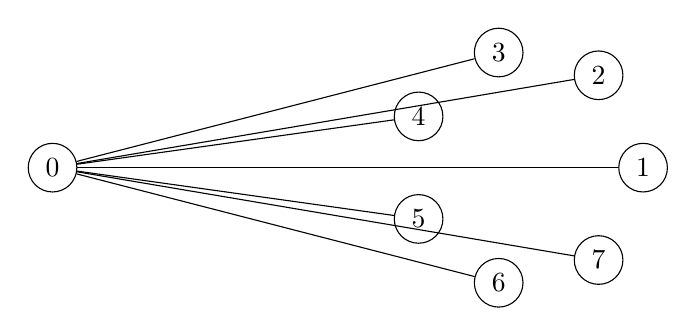
\begin{tikzpicture}
    \draw[every node/.style={circle, draw}]
        (-5, 0) node (0){0}
        (2.5, 0.0) node (1){1}
        (1.935, 1.173) node (2){2}
        (0.666, 1.462) node (3){3}
        (-0.351, 0.651) node (4){4}
        (-0.351, -0.651) node (5){5}
        (0.666, -1.462) node (6){6}
        (1.935, -1.173) node (7){7};
    \begin{scope}[-]
        \draw (0) to (1);
        \draw (0) to (2);
        \draw (0) to (3);
        \draw (0) to (4);
        \draw (0) to (5);
        \draw (0) to (6);
        \draw (0) to (7);
    \end{scope}
\end{tikzpicture}\\
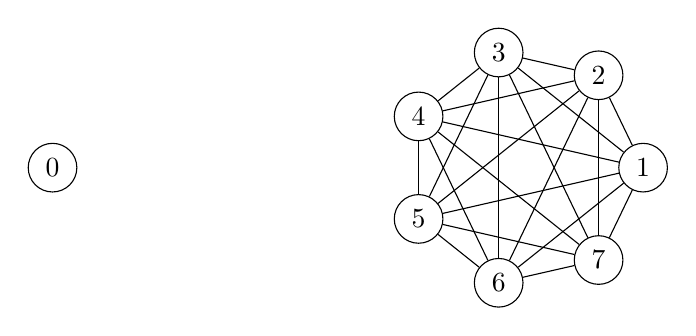
\begin{tikzpicture}
    \draw[every node/.style={circle, draw}]
        (-5, 0) node (0){0}
        (2.5, 0.0) node (1){1}
        (1.935, 1.173) node (2){2}
        (0.666, 1.462) node (3){3}
        (-0.351, 0.651) node (4){4}
        (-0.351, -0.651) node (5){5}
        (0.666, -1.462) node (6){6}
        (1.935, -1.173) node (7){7};
    \begin{scope}[-]
        \draw (1) to (2);
        \draw (1) to (3);
        \draw (1) to (4);
        \draw (1) to (5);
        \draw (1) to (6);
        \draw (1) to (7);
        \draw (2) to (3);
        \draw (2) to (4);
        \draw (2) to (5);
        \draw (2) to (6);
        \draw (2) to (7);
        \draw (3) to (4);
        \draw (3) to (5);
        \draw (3) to (6);
        \draw (3) to (7);
        \draw (4) to (5);
        \draw (4) to (6);
        \draw (4) to (7);
        \draw (5) to (6);
        \draw (5) to (7);
        \draw (6) to (7);
    \end{scope}
\end{tikzpicture}
\end{center}
The picture shows the relation between $S_n$ and $K_n$.

\end{document}
